\section{\'Equipement}

\subsection{Armures}
Voici quelques armure que l’on peu trouver dans l’univers de \swfe. Il s’agit là plus d’une grille d’étalonnage que d’une liste exhaustive. La limite c’est l’imagination des joueurs et la volonté du MJ. Vous trouverez sur \citetitle{website:starwars-holonet} une quantité d’arme décrites dans les moindre détails.

\begin{itemtable}[ X c c c ]
    \textbf{Type} & \textbf{Ar\footnotemark[1]} & \textbf{Pds\footnotemark[2]} & \crg \\
    Veste en Cuir           & +1  & 10 & 50        \\
    Casque                  & +4  &  5 & 80        \\
    Armure Storm Trooper    & +6  & 20 & Militaire \\
    Armure mandalorienne    & +7  & 15 & 1000      \\
    M’uhk’gla (lourde)      & +14 & 30 & 2500      \\
    \hline
    \hline
    Bouclier                & +3  & 20 & 200       \\
    Bouclier Gungan         & +4  & 10 & 1500       
\end{itemtable}

\begin{center}
	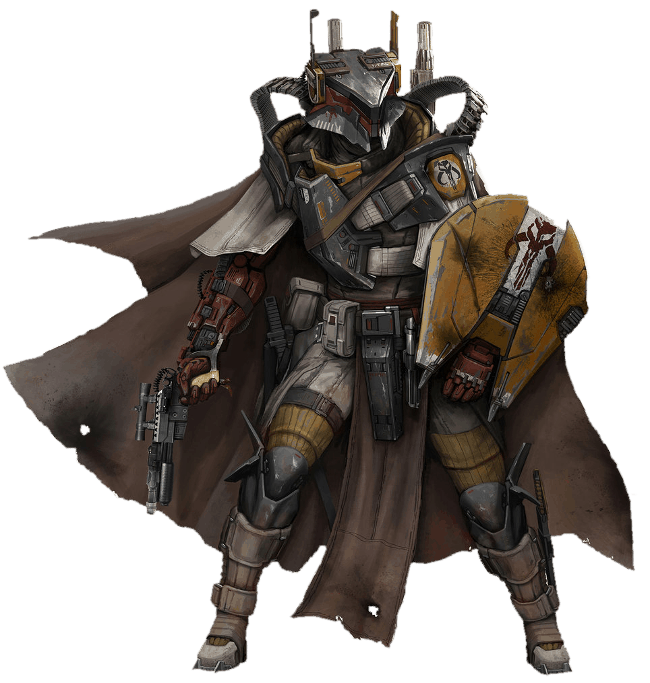
\includegraphics[width=\linewidth]{img/equipement/mandalorian_heavy_armor.png}
	\caption{\emph{Armure lourde Mandalorienne}}
\end{center}

\subsection{Armes}

\subsubsection{Combat corps à corps}

\begin{itemtable}[ X c c c ]
    \textbf{Type} & \textbf{Débats} & \textbf{Pds\footnotemark[2]} & \crg \\
    Vibrolame				& For+d4    &  1 & 25		 \\
    Bâton           		& For+d4    &  1 & 10        \\
    Couteau laser			& 2d6+4     &  1 & 500		 \\
    Vibroépée				& For+d6+2  &  6 & 250		 \\
    Bâton électrique        & For+d8+2  & 10 & 700	
\end{itemtable}

\subsubsection{A distance}

La portée est donné en "case" si le jeux se fait sur table ou sur grille. Une case fait 2.5m, par ex. un Blaster de portée 10 a une portée réelle de 25m.

Entre parenthèse après les légats on trouve la cadence de tir de l’arme. En nombre de projectile maximum envoyé par tour. Attention dés que le nombre de projectile envoyé dépasse 1, il y a un malus de -2 pour le recul.

\begin{itemtable}[ X c c c c ]
    \textbf{Type} & \textbf{Pt\footnotemark[3]} & \textbf{Dégâts} & \textbf{Pds\footnotemark[2]} & \crg \\
    Blaster                 & 10  &  2d6+1 (1) & 4  & 200  \\
    Blaster Lourd           & 15  &  2d8   (1) & 4  & 400  \\
    Fusil Blaster           & 10  &  2d8   (3) & 6  & 800  \\
    Blaster de précision    & 200 &  2d10  (1) & 8  & 1200 \\
    Lance grenade           & 5   &  2d10  (1) & 7  & 500  \\
    Arbalète laser          & 8   &  2d6+1 (3) & 9  & 600  \\
    Canon blaster rotatif   & 20  &  2d8   (4) & 40 & 600
\end{itemtable}

\begin{description}[align=left]
    \item [Fusil Blaster DC-17m]
        Le blaster DC-17m peut être utilisé en trois modèles qui le rendent terriblement efficace pour des missions aussi diverses que celles accomplies par les commandos. Il peut tout d’abord être réglé en mode blaster conventionnel, il possède alors les caractéristiques d’un Fusil Blaster. Le deuxième mode de ce blaster est le mode sniper, il possède alors les caractéristiques d’un Blaster de précision. Enfin, il peut être utilisé en mode grenade, essentiellement pour faire des trous dans les parois blindées et très efficace pour déblayer une zone.

        Le changement de mode prend un tour complet s’il est effectué durant un combat. Cette arme doute 2000\crg.

    \item [Arbalète Laser]
        Cette arme surtout utilisé par les Ewoks et les Wookies est capable d’envoyer jusqu’à 3 projectiles dans des directions différentes sur un même plan horizontal. C’est une arme très lourde qui demande un minimum de For d6+ pour être manipulé correctement.

    \item [Canon blaster rotatif]
        Les armes de ce gabarit nécessite une certaine force pour être utilisé (For d8+). De plus il est impossible de se déplacer lorsque l’on utilise cette arme.
\end{description}

\footnotetext[1]{Armure}
\footnotetext[2]{Poids}
\footnotetext[3]{Portée}

\clearpage
\subsection{Armes Spéciales}

\subsubsection{Sabre Laser}
\label{sec:sabre-laser}

\begin{flushright}
	\vspace{-5\baselineskip}
	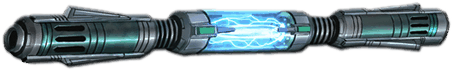
\includegraphics[width=5cm, angle=-25]{img/equipement/lightsaber01.png}
	\vspace{-1\baselineskip}
\end{flushright}

Le sabre laser est l’arme des chevaliers combattant avec la Force, qu’ils soient du Côté Obscur ou du Côté Lumineux. La lame est un faisceau d’énergie pure, produit généralement par trois cristaux polis contenus dans le manche. Seuls les utilisateurs de la Force ont la compétence nécessaire pour l’utiliser. Tout autre utilisateur aurait autant de chances de se blesser que de blesser ses adversaires. 

Il existe une multitude de cristaux à travers la Galaxie, mais seuls certains D’entrés eux, assez rigides, ou bien parfaitement constitués, peuvent être utilisés, et c’est selon les types des cristaux, que la lame arborera une certaine teinte. Chaque cristal peut receler un pouvoir lorsqu’il est alimenté. A travers les âges, beaucoup de ces cristaux furent découverts mais ils sont très rares et difficiles à déceler. En voici quelques exemples : cristal de Solari, cristal Damind, cristal Kaiburr, \ldots

Mais les Jedi arrivèrent également à créer des cristaux industriellement pour alimenter leurs besoins. Ces cristaux peuvent être modifiés lors de leur croissance pour avoir une lame de la couleur voulue, mais toutes les couleurs ne sont pas disponibles. Ces cristaux sont toutefois moins maniables, mais plus puissants que les cristaux naturels qui sont, à l’inverse, plus maniables mais moins puissants. Ce sont, en général, les Sith et les Jedi Noirs qui utilisent ce type de cristaux car ils recherchent la puissance, et non la maniabilité. Historiquement, les Sith ont toujours préféré des lames de couleur rouge. 

Le Sabre laser est une arme très rare, chaque Jedi fabrique le sien et il est unique. Il n’existe doc que deux façons de s’en procurer un, le fabriquer ou le volé sur le cadavre d’un Jedi.

La fabrication d’un Sabre laser n’est pas aisé:
\begin{enumerate}
	\item Trouvé tous les composants, une cellule d’énergie, une lentille, un émetteur de lame et un cristal.
	\item Apprendre les rudiment du montage d’un sabre (Connaissance (Jedi) d6+).
	\item Maîtriser la Force suffisamment pour assembler les différentes pièce (Maîtrise de la Force d6+).
\end{enumerate}

Une fois toutes les conditions remplies, le Jedi doit méditer pendant un mois pour assembler les pièces de son sabre. Quand le sabre est terminé, lors de sa première utilisation, le joueur fait un jet de Maîtrise de la Force, s’il fait 1, le sabre explose, le composant sont perdu et le héro prend un niveau de blessure. Il faudra tout recommencer.

\begin{itemtable}[ X c c c ]
    \textbf{Type} & \textbf{Dégâts} & \textbf{Poids} & \textbf{Notes} \\
    Sabre Laser   & For+d6+8        & 2              & Parade +3, PA 4
\end{itemtable}

\textbf{PA (Pénétration d’armure)}: l’arme ou le projectile ignore les points d’armure indiqués. Une arme avec la capacité PA 4 ignore 4 points d’armure. Les points de PA supérieurs à la protection de la cible sont ignorés.

\begin{center}
	\vspace*{\fill}
	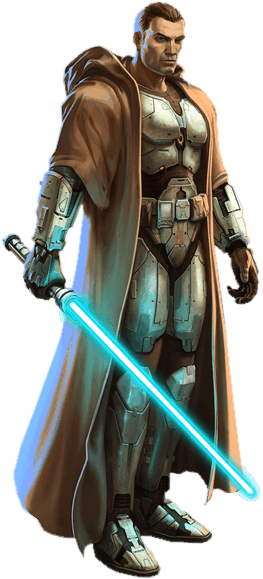
\includegraphics[width=0.7\linewidth]{img/equipement/jedi01.png}
	\vspace*{\fill}
\end{center}

\clearpage
\subsection{Véhicules}
\subsubsection{Armes Embarquées}

La plus part des véhicules peuvent être équipé d’arme plus ou moins lourde. Le nombre d’arme possible dépend de la taille du véhicule et de la volonté du MJ. Le chiffre entre parenthèse indique le nombre de coup que le canon est capable de tirer par tour. Le plasma par exemple à besoin de charger pendant un tour avant de pouvoir tirer.

Comme pour les autres équipement il ne s’agit pas d’une liste exhaustive mais d’exemple qu’il sera possible de faire varier selon les goûts des joueurs et du MJ.

\begin{itemtable}[ X c c c c ]
    \textbf{Type} & \textbf{Porté} & \textbf{Dégâts} & \crg \\
    Canon blaster & 600            & 2d10  (1)       & 100K \\
    Canon ionique & 600            & 4d10  (1)       & 200K \\
    Rail Gun      & 400            & 4d12  (1)       & 400K \\
    Canon laser   & 600            & 7d10  (1)       & 1M   \\
    Canon plasma  & 600            & 10d10 (0.5)     & 10M 
\end{itemtable}

\begin{description}[align=left]
    \item [Rail Gun]
        Ou canon à hyper-vélocité permet aisément de traverser les écrans déflecteurs et s’attaquer directement à la coque de l’unité prise pour cible. Il nécessite des munitions qu’il est facile de se procurer pour 1500\crg ou de miner sur les astéroïdes en 1d6 heures pour 10 munitions.

    \item [Canon ionique]
        Le canon ionique a la particularité de s’en prendre aux systèmes électroniques des vaisseaux sans endommager la coque ou le matériel à l’intérieur, principalement utilisé par les pilleurs pour immobiliser les vaisseaux.
\end{description}


\subsubsection{Véhicules Terrestres}
\footnotetext[1]{Transport Blindé Tout-Terrain}
\footnotetext[2]{Passager}
\footnotetext[3]{Accélération/Vitesse Max}
\footnotetext[4]{Faster Than Light}
\footnotetext[5]{\'Etoile de la mort}
\begin{center}
    \vspace{-2\baselineskip}
    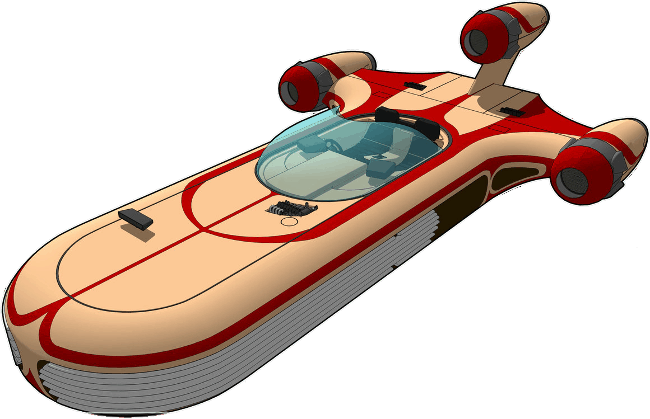
\includegraphics[width=0.9\linewidth]{img/equipement/landspeeder.png}
    \vspace{-1\baselineskip}
\end{center}

\begin{itemtable}[ X c c c c ]
    \textbf{Type} & \textbf{Acc/VMax} & \textbf{Rés.} & \textbf{Pger\footnotemark[2]} & \crg \\
    Motojet         & 20/36           & 8(2)          & 1+1               & 6 000  \\
    Landspeeder     & 20/40           & 11(3)         & 1+3               & 12 000 \\
    Podracer        & 30/56           & 10(3)         & 1                 & 25 000 \\
    TB-TT\footnotemark[1] & 5/16 & 110(100) & 2+40 & Militaire 
\end{itemtable}

\subsubsection{Véhicules Aériens}
Les véhicules aérien sont pour la plus part man\oe{uvrable} en haute atmosphère mais ne permettent pas de voyage FTL\footnotemark[4]. 
\begin{center}
    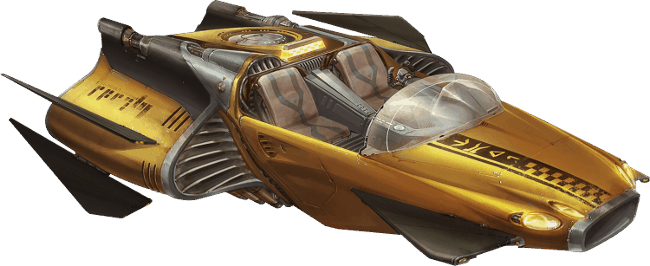
\includegraphics[width=0.9\linewidth]{img/equipement/airspeeder-taxi.png}
\end{center}
\begin{itemtable}[ X c c c c ]
    \textbf{Type} & \textbf{A/VM\footnotemark[3]} & \textbf{Rés.} & \textbf{Pger\footnotemark[2]} & \crg \\
    Air Speeder     & 20/40           & 16(4)         & 1+1               & 60 000
\end{itemtable}

\subsubsection{Vaisseaux Spatiaux}
Tous ces vaisseaux possèdent la navigation FTL.
\begin{itemtable}[ X c c c c ]
    \textbf{Type} & \textbf{Acc/VMax} & \textbf{Rés.} & \textbf{Pger\footnotemark[2]} & \crg      \\
    Chasseur                & 50/700           & 20(5)         & 1+1               & 2M        \\
    Navette                 & 45/600           & 25(6)         & 2+5               & 5M        \\
    Transport               & 35/400           & 45(10)        & 2+20              & Militaire \\
    Croiseur                & 30/300           & 50(11)        & 15+985            & 200M      \\
    Bâtiment                & 25/200           & 55(13)        & 20+2980           & Militaire \\
    EDLM\footnotemark[5] & 20/200  & 80(25)      & 100+5K            & Militaire 
\end{itemtable}

\begin{center}
    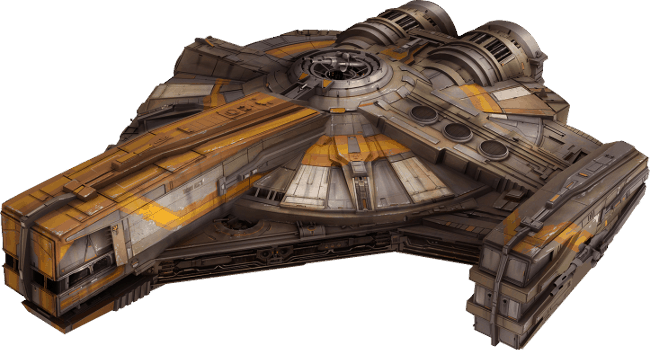
\includegraphics[width=0.9\linewidth]{img/equipement/navette.png}
\end{center}

\begin{description}[align=left]
    \item [Chasseur léger]
        Beaucoup de vaisseaux rentrent dans cette catégorie. Le X-Wing, le Tie, ...

    \item [Navette]
        Dans cette catégorie rentre les vaisseaux comme le Millenium Falcon ou le Slave 1.

    \item [Croiseur]
        Beaucoup plus rare dans les campagnes mais les MJ peuvent s’en servir.

    \item [Bâtiment]
        Il s’agit des Battleships, vaisseaux de grande taille, capable d’en contenir d’autres (type chasseur). Lourdement armé la plus part du temps. Le Destroyer Impérial se classe dans cette catégorie.

    \item [Station Orbitale]
        Juste pour la forme car rarissime dans les campagnes de jeux. Les stations orbitales sont capable de détruire des planètes entières.
\end{description}

\onecolumn
\begin{figure}
  \caption{Croiseur}
  \centering
  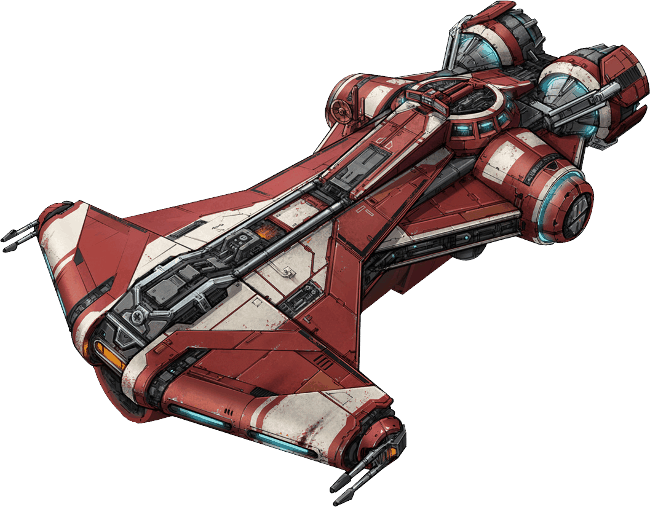
\includegraphics[width=0.8\textwidth]{img/equipement/croiseur.png}
\end{figure}
\begin{figure}
  \caption{Bâtiment}
  \centering
  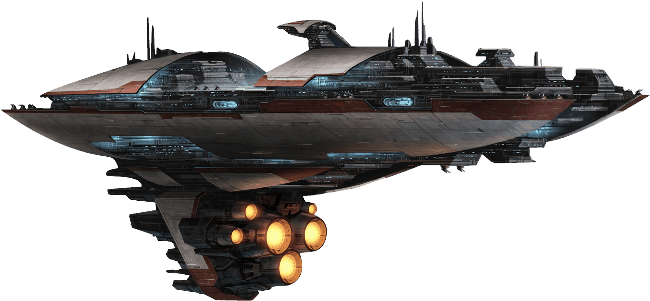
\includegraphics[width=0.9\textwidth]{img/equipement/batiment.png}
\end{figure}
\twocolumn